% Marco Teorico.
\chapter{Marco te'orico} \label{chap:ssimilar}



Los conceptos claves acerca de ERP, SAP, ABAP son los que se presentan en este capítulo.
\newline
\newline
La secci'on ~\ref{sect:erp} presenta las nociones b'asicas acerca de en qu'e consiste un Sistema de Informaci'on ERP. La secci'on 
~\ref{sect:sap} describe un poco lo que es SAP: sus caracter'isticas principales, una  breve historia. Por otro lado, la secci'on ~\ref{sect:abap} explica en que consiste el lenguaje de programaci'on ABAP, sus principales caracter'isticas. 

\section{ ERP} \label{sect:erp}


\subsection{Definiciones} \label{subsect:defprop}


Seg'un Kogent(2006), un ERP (Sistema de Planificación de Recursos Empresariales, o como se le conoce en Ingl'es: \textbf{Enterprise Resource Planning}), es un sistema que tiene la capacidad de la automatizaci'on e integraci'on de todos los m'odulos de un 'area de negocio. En otras palabras, es capaz de manejar todas las 'areas relacionadas con una empresa de forma automatizada e integrada. 
\newline
\newline
\indent Seg'un Cruz-Cunha(2010), ella hace referencia a (Miller, 2002), quien define a ERP  como "un m'etodo para la planeaci'on efectiva y control de todos los recursos necesitados para tomar, hacer, entregar las 'ordenes de los clientes dentro de una compa\~nia dde manufactura, distribuci'on o servicios''. De acuerdo a la autora, un sistema ERP intenta integrar todos los departamentos y sus respectivos m'odulos de aplicaciones dentro de un sistema cuyo fin es satisfacer las necesidades de dichos departamentos como un repositorio central. 
\newline
\newline
\indent Seg'un Cruz-Cunha(2010), la principal diferencia entre un sistema ERP y un sistema convencional consiste en que los m'odulos que componen al sistema ERP est'a enlazado a una Base de Datos com'un, con lo cual se elimina la necesidad de tener entradas m'ultiples de datos, lo que conlleva a redundancia. Los sistemas convencionales, por otro lado, tienen su propia Base de Datos, con lo cual se tienen los problemas que un ERP evita.
Una caracter'istica fundamental de este tipo de sistemas es que est'a basado en m'odulos. 
\newline
\newline
\indent Segun Kogent(2006), otra ventaja que poseen los sistemas ERP, es que este ayuda a sincronizar los datos y los mantiene actualizados.
\subsubsection{Beneficios que aporta los Sistemas ERP}
	Seg'un Hamilton(2003), los beneficios que un sistema ERP est'an relacionados con el inventario y los materiales, el trabajo y sus costos, el servicio al cliente y las ventas. Estos son los que se listan a continuaci'on:
\begin{enumerate}
\item Reducci'on de Inventario
\item Reducci'on de Costos en Materiales
\item Reducci'on de Costos en trabajo
\item Mejoras en el Servicio al Cliente y las ventas
\end{enumerate}
\subsubsection{Desventajas de un Sistema ERP}
\indent De acuerdo con Kogent(2006), los sistemas ERP poseen varias desventajas. Algunas de estas son las que se citan a continuaci'on:
\begin{itemize}
\item La adaptaci'on de un sistema ERP es restringido, dado que no es sencillo adaptarlos a un flujo espec'ifico de trabajo o a un proceso de negocio de una compa\~nia.
\item Una vez que un sistema ERP es instalado, la migraci'on a otro sistema de este tipo es costoso.
\end{itemize}
\section{SAP} \label{sect:sap}


\subsection{Definici'on} \label{subsect:defprop}
	 Por su origen alem'an, las siglas SAP son un acr'onimo de: \textit{Systeme, Anwendungen Produkte in der Datenverarbeitung}, que traducido al castellano significa: \textbf{Sistemas, Aplicaciones y Productos en Procesamiento de Datos}. (Kogent (2006))
\newline
\newline
\indent De acuerdo a Sharma y Mutsaddi(2010), el Software principal desarrollado por esta empresa es \textbf{\textit{SAP R/3}} y el cual se encuentra disponible en 28 idiomas. Este software es personalizable, utiliza la arquitectura cliente-servidor. Este software fue hecho en el lenguaje de programaci'on \textbf{ABAP/4}. 

\subsection{Caracter'isticas de SAP R/3}
Seg'un Khan(2002), las caracter'isticas del software \textbf{SAP R/3} se pueden dividir en diferentes categor'ias, las cuales se mencionan a continuaci'on:

\subsubsection*{Caracter'isticas Generales}
\begin{itemize}
\item Es un software altamente integrado y multifuncional, lo que trae como consecuencia que exista una estrecha relaci'on entre las funciones del mismo.
\item Es una aplicaci'on que trabaja en tiempo real. En otras palabras, las actualizaciones de los datos son efectuadas a trav'es de una conexi'on, y en ese mismo instante.
\end{itemize}
\subsubsection*{Caracter'isticas de Negocio}
\begin{itemize}
\item Contiene todas las funcionalidades necesarias para poder llevar a cabo el manejo de un negocio entero. Adem'as que ncorpora una aplicaci'on llamada \textit{Best Industry Practices}, que traducido al espa\~nol quiere decir: \textit{Mejores Practicas de la Industria}, y 'este 'ultimo es adecuado para una amplia gama de industrias y organizaciones.
\item Es capaz de soportar todos los procesos de negocio de la empresa.
\end{itemize}

\subsubsection*{Caracter'isticas de Flexibilidad}
\begin{itemize}
\item Es altamente configurable. En otras palabras, se puede adaptar a las necesidades de la empresa que lo utilice y a sus requerimientos. Para ello, se pueden realizar cambios que, dependiendo del n'umero de factores que participen, 'estos tendr'an su grado de complejidad.
\item Es capaz de dar apoyo a empresas que poseen subsidiarias en distintas partes del mundo.
\end{itemize}

\subsubsection*{Caracter'isticas T'ecnicas}
\begin{itemize}
\item Tiene la capacidad de ser portable, dado que es multiplataforma, es decir, soporta cualquier sistema operativo, manejador de Base de Datos, etc.
\item Posee un n'umero m'inimo de redundancia, lo que favorece a la consistencia de los datos almacenados. Adicionalmente, posee un manejador de alta seguridad de los datos, y puede manejar etructuras de datos complejas.
\end{itemize}

\subsubsection*{Otras Caracter'isticas}
\begin{itemize}
\item Tiene la capacidad de manejar la misma informaci'on en cada m'odulo.
\item Posee una 'unica manera de ingreso al sistema. Esta es a trav'es del \textit{SAP GUI}.
\item Tiene la capacidad de ser escalable, es decir, que est'a preparado para manejar el continuo crecimiento del trabajo sin disminuir la calidad.
\item Tiene una interfaz gr'afica amigable.
\end{itemize}

\subsection{Adaptaci'on del Software a las Empresas}
Seg'un Khan (2002), para poder realizar la adaptaci'on de SAP a las necesidades de una empresa en particular, se cuenta con un conjunto de herramientas y utilidades destinadas a ello. Para esto, se requiere de un conjunto de consultores, un equipo de proyecto y personal de Tecnolog'ia de la Informaci'on (IT por sus siglas en ingl'es), quienes ser'an los encargados de efectuar dicha adaptaci'on. 
\newline
\newline
Este proceso se puede realizar a trav'es de dos m'etodos, los cuales se listan a continuaci'on:

\begin{itemize}
\item \textbf{Cambios en la Configuraci'on:} Aqu'i son modificadas las tablas relacionadas con los distintos m'odulos para poder realizar la adaptaci'on.
\item \textbf{Programaci'on en el Lenguaje ABAP/4:} Esto implica modificar programas ya existentes en \textbf{SAP R/3} o crear programas nuevos.
\end{itemize}


\section{M'odulo de Ventas y Distribuci'on (SD)} \label{sect:sd}

Seg'un Kogent (2011), el \textbf{M'odulo de Ventas y Distribuci'on} (Sales and Distribution como es conocido en ingl'es) es un sub-sistema perteneciente a SAP, el cual se encarga de prestar apoyo a las distintas empresas en el 'area de las Ventas y distribuci'on de productos y/o servicios. 
\newline
\newline
\indent Seg'un Kogent (2011), este m'odulo ayuda a las compa\~n'ias a establecer un precio para sus productos, chequear 'ordenes de ventas que se mantienen abiertas, a tomar previsiones para necesidades futuras, etc. Adicionalmente, ayuda a dar mayor control a las actividades relacionadas con el 'area de ventas: desde el momento en que ocurre un pedido de alg'un(algunos) producto(s) y/o servicio(s) hasta su posterior entrega.



\subsection{Componentes Principales}
	Segun Kogent (2011), dentro del M'odulo de Ventas y Distribuci'on (SD), se cuenta con un numeroso n'umero de componentes, los cu'ales facilitan el trabajo en 'esta 'area. En los pr'oximos apartados se explican cada uno.
\subsubsection{Manejo de Precios e Impuestos}
A trav'es de esta herramienta, el m'odulo puede evaluar los precios que son colocados a los productos o servicios de acuerdo a unas condiciones establecidas previamente. 
\subsubsection{Chequeo de Disponibilidad}
Con esta herramienta, el m'odulo puede evaluar la disponibilidad de un producto para un almac'en especificado.
\subsubsection{Manejo de Cr'edito}
Con esta herramienta es posible establecer l'imites de cr'edito para un cliente durante el proceso de ventas en el cual se encuentra envuelto.
\subsubsection{Facturaci'on}
Una vez que una Orden de Ventas es creada, se utiliza esta herramienta para crear la(s) factura(s) asociadas.
\subsubsection{Determinaci'on del Material}
Con esta herramienta es posible determinar un material específico de acuerdo a unas condiciones especificadas.
\subsubsection{Determinaci'on de Cuentas}
Ayuda a obtener ciertos detalles de los clientes bas'andose en unas condiciones espec'ificas.
\subsubsection{Procesamiento de Textos}
Con esta herramienta se hace posible el manejo de textos entre los distintos documentos que se obtienen del proceso de ventas.


\subsection{Clasificaci'on de los Datos en el M'odulo SD}
Seg'un Kogent (2011), la data almacenada dentro del M'odulo se clasifica como se muestra en la figura ~\ref{fig:datasd} donde se muestra la siguiente clasificaci'on:
\begin{figure}[H]
\centering
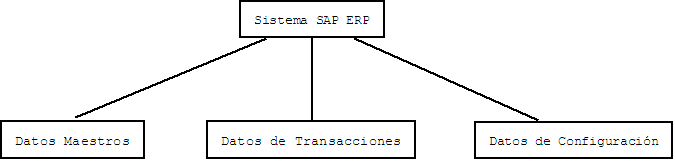
\includegraphics[scale=0.70,type=png,ext=.png,read=.png]{figures/Clasificacion1}
\caption{Clasificaci'on de los datos en el M'odulo SD}
\label{fig:datasd}
\end{figure}
\subsubsection*{Datos Maestros}
Los Datos Maestros dentro del M'odulo SD est'an compuestos por: Datos de Compa\~n'ias y Datos Maestros de Clientes
Cada una de estas entidades contiene a su vez atributos, jerarqu'ias y tablas.

\subsection{Proceso de Ventas utilizando el M'odulo SD}
\indent Seg'un Kogent (2011), en este m'odulo los dos objetos m'as importantes son: las clases de documentos y las condiciones. El primero, porque en cada fase del proceso se elabora un documento que contiene informaci'on relevante para dicha fase. La segunda, porque contiene las cl'ausulas por las cuales se va a regir el esquema de precios.
\newline
\newline
\indent En las tablas ~\ref{tb:procesoventas} y ~\ref{tb:procesosd3}, se detalla cada una de las etapas presentes en el proceso de ventas del m'odulo SD.

\begin{table}[H]
\footnotesize
\begin{tabular}{|l|l|}
\hline
\textbf{Nombre del Proceso}  & \textbf{Descripci'on}  \\
\hline
Solicitud de Informaci'on de Productos & Este es el punto de partida para el proceso de ventas. \\
                                                            & En este paso, el cliente solicita informaci'on acerca de \\
                                                            & los productos y/o servicios que son ofrecidos por la em - \\
                                                            & presa, con el objetivo de una posible adquisici'on de al - \\
                                                            & g'un producto y/o servicio. \\
\hline
Creaci'on de Orden de Ventas               & En este punto, el cliente le solicita a la empresa un pedi -\\ 
                                                            & do de un material determinado solicitado en el paso ante -\\
                                                            & rior. Para esto, se crea en SAP lo que se conoce como un \\ 
                                                            & \textbf{Pedido de Venta}. Un \textbf{Pedido de Venta} es \\
                                                            & un documento que contiene informaci'on acerca del(los) \\
                                                            & material(es) que se est'a solicitando, entre otras cosas. Un \\
                                                            & Pedido tiene la siguiente divisi'on: \\
                                                            & - \textbf{Cabecera del Documento:} En esta parte del docu -\\
                                                            & mento se recoge informaci'on acerca de la informaci'on gen -\\
                                                            & eral del pedido. Entre la informaci'on relevante que se puede \\
                                                            & encontrar, se pueden mencionar: \\
                                                            & 1. Fecha del Pedido \\
															  & 2. Cliente que hace el Pedido \\
															  & 3. Cliente que recibe el Pedido \\
															  & 4. Tipo de Pedido (Si es un Pedido est'andar, Contrato con el \\
															  & cliente, solicitud de Nota de Cr'edito/D'ebito, Retorno de Pro -\\
															  & ductos, Consulta de Cliente, solicitud de Presupuesto) \\
															 & 5. N'umero de Pedido: El el n'umero con el cual el cliente iden -\\
															 & tifica su pedido. \\
															 & N'umero de Documento: Es el n'umero con el cual se identifica\\
															 & un'ivocamente el Pedido de Ventas.\\
															 & - \textbf{Posiciones del documento:} Contiene informaci'on so -\\
															 & bre los materiales solicitados. Cada material va colocado en una \\
															 & posici'on diferente, y en 'esta se reflejan los siguientes datos:\\
															 & 1. N'umero de Material: Es el n'umero que identifica un'ivo -\\
															 & camente al material solicitado. \\
															 & 2. Descripci'on del Material: Es un nombre que se le coloca al\\
															 & material.\\
															 & 3. Cantidad\\
															 & 4. Unidad de Venta: Es la unidad en la cual se vende el material.\\
															 &  Esto ocurre porque dentro de la informaci'on que posee el ma -\\
															 & terial, se diferencian dos unidades: la de almacenamiento y la \\
															 & de venta \\
															 & 5. Precio bruto: Es el precio del material. \\
															 & Para esto se tienen las siguientes transacciones, las cuales son \\
															 & las m'as utilizadas:\\
															 & - VA01: Creaci'on de Pedidos \\
															 & - VA02 Modificaci'on de Pedidos \\
														     & - VA03: Visualizaci'on de Pedidos \\
\hline
\end{tabular}
\caption{Proceso de Ventas - Parte 1(Informaci'on obtenida de Sharma y Mutsaddi (2010))}
\label{tb:procesoventas}
\end{table}
\begin{table}[H]
\footnotesize
\begin{tabular}{|l|l|}
\hline
\textbf{Nombre del Proceso}  & \textbf{Descripci'on}  \\
\hline
Entrega de Bienes y/o Servicios            & El segundo paso a ejecutar una vez que se cre'o el pedido de ventas,\\
                                                            & es la creaci'on de una  Entrega. Para esto, se crea un nuevo documen -\\
                                                            & to el cual es llamado \textbf{Documento de Entrega}. Esto es, porque\\
                                                            & en el mencionado documento, se detalla la informaci'on relacionada\\
                                                            & con el proceso de entrega y transporte. En este documento, adem'as de\\
                                                            &  la informaci'on que es copiada del documento anterior (Cabecera y Po -\\
                                                            & siciones), se detalla informaci'on acerca de las cantidades reales entrega -\\
                                                            & das, ya que las cantidades solicitadas en el Pedido est'an sujetas a la dis -\\
                                                            & ponibilidad de las mismas en los Almacenes. Para ello, es necesario el uso\\
                                                            & de las siguientes transacciones:\\
															  & - VL01N: Creaci'on de Entregas\\
															  & - VL02N: Modificaci'on de Entregas\\
															  & - VL03N: Visualizaci'on de Entregas\\
															  & Una vez que la entrega es creada, se debe contabilizar el material, para que\\
															  & la entrega est'e considerada como completada. Esto es, para que pueda\\ 
															  & procederse al siguiente paso.\\
\hline
Facturaci'on             							  & La siguiente acci'on a realizar dentro del ciclo es la facturaci'on. En\\ 
															  & este paso, como su nombre lo indica, se crea la factura relacionada con\\ 
															  & un pedido previamente realizado. En este documento, se reflejan los ma -\\
															  & teriales y/o servicios solicitados, con sus respectivas cantidades y su monto.\\ 
															  & Adicionalmente, es  reflejado los impuestos que apliquen, asi como  el monto\\
															  & total a pagar por el solicitante. Para esto, es necesario el uso de las\\ 
															  & siguientes transacciones:\\
															  & - VF01: Creaci'on de Facturas\\
															  & - VF02: Modificaci'on de Facturas\\
															  & - VF03: Visualizaci'on de Facturas\\
															  & Es posible, en primer lugar, la creaci'on de varias facturas. Esto es\\ 
															  & posible gracias a las negociaciones que lleva la empresa con el cliente,\\
															  &  sobre los montos a pagar. En segunda instancia, si hubo errores en la\\
															  &  factura creada, es posible la anulaci'on de la misma, con lo cual la deuda\\ 
															  & adquirida por el cliente se anula, en caso de no tener otra factura pen -\\  
															  & diente. Con eso es posible volver a crear la factura con las correcciones\\
															  &  a aplicar. Una vez creada la factura, se debe contabilizar la misma. Esto\\
															  & es con el fin de que se cree un documento contable, para que la nueva\\ 
															  & venta est'e reflejada dentro de la contabilidad de la empresa.\\
\hline
Pago por los bienes y/o servicios& Este es el paso final del ciclo de ventas que es  llevado en el m'odulo SD. Para\\ 
adquiridos				                    & ello, de acuerdo a los planes de pago establecidos entre la empresa y el cliente,\\ 
                                                   & la misma inicia el cobro de la deuda adquirida.\\
\hline
\end{tabular}
\caption{Proceso de Ventas - Parte 2 (Informaci'on obtenida de Sharma y Mutsaddi (2010))}
\label{tb:procesosd3}
\end{table}

\subsection{Relaci'on existente entre el M'odulo SD y otros M'odulos}
De acuerdo a Kogent (2011), este m'odulo est'a fuertemente integrado con otros m'odulos de SAP, como por ejemplo: MM, WM, QM. 
\newline
\newline
\indent En el momento en que un cliente realiza un pedido de alg'un producto, posteriormente se chequea la disponibilidad del mismo en alg'un almac'en; esto es posible gracias al m'odulo MM. 
\newline
\newline
\indent Por otro lado, el m'odulo QM es el encargado de manejar la calidad y brindar soporte a un servicio prestado al cliente, ambos representados por un documento de ventas en SD. 

\section{Lenguaje de Programaci'on ABAP/4} \label{sect:abap}
De acuerdo a Kogent (2011), ABAP (Advanced Business Application Programming - Programaccion de Aplicaciones de Negocio Avanzado) es un lenguaje de programaci'on que fue dise\~nado en la d'ecada de los 80. Su uso principal es la de generar reportes con los cuales se les permite a las empresas construir sus propias aplicaciones para el manejo de las distintas 'areas que lo componen (manejo de materiales, manejo del 'area financiera, manejo de las ventas, etc).
\newline
\newline
Seg'un Kogent (2011), este es uno de los primeros lenguajes de programación que incluye dentro de su definición el concepto de Bases de Datos L'ogicas. 
\newline
\newline
Seg'un Kogent (2011), dentro de las caracter'isticas que posee el lenguaje, se pueden mencionar las siguientes:
\begin{itemize}
\item Es un lenguaje basado en la programaci'on estructurada. En otras palabras, contiene estructuras de control.
\item Es un lenguaje interpretado, aunque existen versiones compiladas del mismo.
\item Es muy utilizado para obtener dos tipos de programas: los que son usados para obtener por ejemplo un listado (modo reporte), y aquellos que son usados como transacciones (modo di'alogo).
\item Es un lenguaje orientado a eventos, es decir, que puede ser controlado desde el exterior a trav'es de sentencias de eventos.
\item Est'a integrado totalmente con el sistema \textbf{SAP R/3}.
\item La salida de sus programas es multilingual. 
\end{itemize}

	
\subsection{Herramientas provistas por ABAP/4}
	Seg'un Kogent (2011), dentro de las herramientas m'as utilizadas de \textbf{ABAP/4}, est'an las que se listan a continuaci'on:
\begin{itemize}
\item Smartforms (Formularios)
\item Sesiones de Batch Input (Carga masiva de datos)
\end{itemize} 
	En la siguientes subsecciones se explicar'a m'as a detalle acerca de dichas herramientas.
	
\subsubsection{Smartforms}
	Seg'un Kogent (2011), \textbf{Los Smartforms} fueron introducidos dentro del lenguaje a trav'es de la versi'on 4.6 de \textbf{SAP R/3}. Su funci'on principal es la impresi'on y env'io de documentos a trav'es del correo electr'onico, o por fax. 
\newline
\newline
\indent Seg'un Kogent (2011), con esta herramienta es posible hacer el dise\~no de formularios, archivos PDF y documentos en general. 
\newline
\newline
\indent Seg'un Kogent (2011), Esta herramienta provee una interfaz capaz de construir y mantener la disposici'on y l'ogica del formulario.
\newline
\newline
\indent Seg'un Kogent (2011), Una ventaja que tiene esta herramienta es el uso  de una interfaz gr'afica para modificar formularios, ya que con esto, se evita el uso de la programaci'on.
\newline 
\newline
\indent Seg'un Kogent (2011), en un smartform, los datos son transmitidos a trav'es de t'ablas din'amicas o est'aticas. Adicionalmente permite incluir gr'aficos que pueden ser visibles en el formulario. En los pr'oximos segmentos se explicar'a los componentes de esta herramienta.
	
\subsubsection{Sesi'on de Batch Input (Carga Masiva de Datos)}
	Seg'un Kogent (2011), esta es una herramienta que provee ABAP/4 con el fin de introducir datos de manera no interactiva dentro del Sistema SAP. La Carga Masiva o por Lotes (Batch Input) es usuado muy frecuentemente para transferir datos desde sistemas externos a un sistema SAP, o entre sistemas SAP. Una sesi'on de Batch Input, m'as espec'ificamente, es un conjunto de una o varias llamadas a transacciones con los datos a ser procesados por dichas transacciones.  
\newline
\newline
	Para poder lograr esta tarea, existen dos transacciones en SAP: la SHDB y la SM35. A partir de la ejecuci'on de alguna de las transacciones antes mencionadas, el sistema se encarga de realizar una grabaci'on sobre la(s) transacción(es) involucrada(s) junto con los datos en un formato especial el cuan puede ser interpretado por SAP. Cuando el sistema ejecuta una sesi'on, utiliza los datos almacenados en dicha sesi'on para comenzar la simulaci'on de la entrada on-line de los datos. El sistema llama a las transacciones y carga los datos en ella. En la Figura~\ref{fig:process}  se puede apreciar los pasos a seguir para poder llevar a cabo una sesi'on de Batch Input. Para ello, el sistema a trav'es de una interfaz recibe el archivo que contiene los datos a ser cargados, y este es pasado al programa de Carga Masiva (Batch Input), el cual se encarga de procesar dichos datos y colocarlos en una cola, para luego procesar uno por uno a trav'es de la simulaci'on de la ejecuci'on de la transacci'on involucrada. 
	
\begin{figure}[H]
\centering
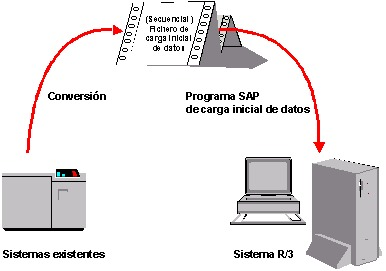
\includegraphics[scale=1.25,type=jpg,ext=.jpg,read=.jpg]{figures/batchinput}
\caption{Proceso de Batch Input ejecutado en SAP (Informaci'on obtenida de la p'agina web de ayuda de SAP)}
\label{fig:process}
\end{figure}


